	
\documentclass[review]{elsarticle}
\usepackage{hyperref,lineno}
\usepackage{xcolor}
\modulolinenumbers[5]

\newcommand{\memo}[2]{\textcolor{#1}{#2}}
\newcommand{\xavi}[1]{\memo{orange}{xavi: #1\\}}
\newcommand{\maria}[1]{\memo{blue}{maria: #1\\}}
\journal{Journal of \LaTeX\ Templates}

%%%%%%%%%%%%%%%%%%%%%%%
%% Elsevier bibliography styles
%%%%%%%%%%%%%%%%%%%%%%%
%% To change the style, put a % in front of the second line of the current style and
%% remove the % from the second line of the style you would like to use.
%%%%%%%%%%%%%%%%%%%%%%%

%% Numbered
%\bibliographystyle{model1-num-names}

%% Numbered without titles
%\bibliographystyle{model1a-num-names}

%% Harvard
\bibliographystyle{model2-names.bst}\biboptions{authoryear}

%% Vancouver numbered
%\usepackage{numcompress}\bibliographystyle{model3-num-names}

%% Vancouver name/year
%\usepackage{numcompress}\bibliographystyle{model4-names}\biboptions{authoryear}

%% APA style
%\bibliographystyle{model5-names}\biboptions{authoryear}

%% AMA style
%\usepackage{numcompress}\bibliographystyle{model6-num-names}

%% `Elsevier LaTeX' style
%\bibliographystyle{elsarticle-num}
%%%%%%%%%%%%%%%%%%%%%%%

\begin{document}

\begin{frontmatter}

\title{Another glass of failure? \tnoteref{mytitlenote}}

%\tnotetext[mytitlenote]{Fully documented templates are available in the elsarticle package on \href{http://www.ctan.org/tex-archive/macros/latex/contrib/elsarticle}{CTAN}.}

%% Group authors per affiliation:
%\author{Mar\'ia Coto-Sarmiento\fnref{myfootnot}}
\author[bscadress]{Maria Coto-Sarmiento \corref{mycorrespondingauthor}}
\author[edadress]{Xavier Rubio-Campillo}
\author[ceipacadress]{Jos\'e Remesal}

%\address{Radarweg 29, Amsterdam}
%\fntext[myfootnote]{Since 1880.}

%% or include affiliations in footnotes:
%\author[mymainaddress,mysecondaryaddress]{Elsevier Inc}
%\ead[url]{www.elsevier.com}

%\author[mysecondaryaddress]{Maria Coto-Sarmiento\corref{mycorrespondingauthor}}
\cortext[mycorrespondingauthor]{Corresponding author}
\ead{maria.coto@bsc.es}

\address[bscadress]{Barcelona Supercomputing Center (BSC), Barcelona, Spain}
\address[edadress]{University of Edinburgh, UK}
\address[ceipacadress]{CEIPAC, University of Barcelona, Barcelona, Spain}
\begin{abstract}
%This template helps you to create a properly formatted \LaTeX\ manuscript.
\end{abstract}

\begin{keyword}Cultural Evolution, Roman Empire, amphorae production, social learning
\end{keyword}

 \end{frontmatter}

\linenumbers

%\section{The Elsevier article class}

%\paragraph{Installation} If the document class \emph{elsarticle} is not available on your computer, you can download and install the system package \emph{texlive-publishers} (Linux) or the \LaTeX\ package \emph{elsarticle} using the package manager of your \TeX\ installation, which is typically \TeX\ Live or Mik\TeX.

%\paragraph{Usage} Once the package is properly installed, you can use the document class \emph{elsarticle} to create a manuscript. Please make sure that your manuscript follows the guidelines in the Guide for Authors of the relevant journal. It is not necessary to typeset your manuscript in exactly the same way as an article, unless you are submitting to a camera-ready copy (CRC) journal.

%\paragraph{Functionality} The Elsevier article class is based on the standard article class and supports almost all of the functionality of that class. In addition, it features commands and options to format the
%\begin{itemize}
%\item document style
%\item baselineskip
%\item front matter
%\item keywords and MSC codes
%\item theorems, definitions and proofs
%\item lables of enumerations
%\item citation style and labeling.
%\end{itemize}

%\section{Front matter}
%The author names and affiliations could be formatted in two ways:
%\begin{enumerate}[(1)]
%\item Group the authors per affiliation.
%\item Use footnotes to indicate the affiliations.
%\end{enumerate}
%See the front matter of this document for examples. You are recommended to conform your choice to the journal you are submitting to.


\section{Introduction}

Material culture allows to understand a part of the mechanism of the human behavior \citep{richerson2005not, schillinger_copying_2016}. This mechanism has been analyzed by the study of variability on material culture which can help us to detect social learning patterns as for instance how to teach and make an amphora. The detection of those patterns in artefact production in the archaeological records could also explain whether these changes are produced by cultural reasons which varying over time and space \citep{basalla1988evolution}. As result, different information are shared by social learning generating an accumulation of knowledge which are transmitted from generation to generation in different context and content conditions \citep{eerkens_jelmer_cultural_2005, neff1992ceramics,henrich_evolution_2003, boyd_cultural_2011}. In any case, the mode of learning transmission along with several external conditions might affect directly or indirectly the pattern of manufacturing of the artefacts.

\xavi{Por otra parte, quien es tu publico, los arqueologos de roma o los que hace arqueologia evolutiva? Porque quedarte en medio no funciona...decide uno de los 2 targets y leete el paper como si fueras o mesoudi o wilson, vaya.}

This paper explores the changes in the production processes during the Roman Empire. In particular, our study is focused on understanding the pottery-making techniques by analyzing large-scale amphorae production in a specific area. In this case, an evolutionary framework is used for studying the implication and the impact that this production might involve on the  evolution of social learning processes. Within evolutionary perspective, social learning is analyzed to understand the human behaviour in archaeology. Thought material culture, we can observe cultural patterns which can explain how the culture evolve \citep{richerson2005not}. Specifically, the aim of this study is understanding how the amphorae production were organized and whether it is possible to identify amphorae made in different workshops. Our main hypothesis concerns about understanding the modes of transmission of pottery-making techniques and how these techniques could have been transmitted in time and space. 

Following a large number of authors \citep{cavalli-sforza_cultural_1981, hosfield_modes_2009}, pottery production can be learned on different modes of cultural transmission depending on the level of production in the communities. Vertical transmission is a mode of transmission when the teaching of the production is done from master to disciple while in horizontal transmission individuals teach pottery techniques to others individuals within the same level and those workers spread the knowledge to their community \citep{epstein_craft_1998}

%cambiar artifact variation// quizas meter producción en masa aquí relacionada con la variacion del artefacto... ??? 

 In material culture, artefact variation might be affected by geographical distance \citep{bjorklund_effect_2010,shennan_isolation-by-distance_2015, van_strien_isolation-by-distance_2015} where material culture is more similar in close population who interacted each other. In other case, the correlation between both seems not visible due to different factors \citep{hart_effects_2012}. 
%podría extender un poc omás con el paper de boyd y richerson



%Specifically, the aim of this study is understanding if pottery-making techniques were transmitted through vertical or horizontal social learning. Our main hypothesis concerns the transmission of the techniques by vertical transmission and how vertical transmission is spreading in time and space. These technological knowledges could have been transmitted from master to disciple and thus continuously. If vertical transmission predominates in this process over horizontal transmission then amphorae made in nearby workshops might share more similar traits than amphorae made from farthest workshop. Otherwise whether horizontal transmission is the main transmission in this process the social learning would be transmitted by workers. Then there would not be differences among workshops on the production. The artefact variation can be related to the geographical distance \citep{bjorklund_effect_2010,shennan_isolation-by-distance_2015, van_strien_isolation-by-distance_2015}. In material culture, artefact variation might be affected by geographical distance where material culture is more similar in close population who interacted each other. In other case, the correlation between both seems not visible due to different factors \citep{hart_effects_2012}. In our case, we can detect measurable differences among this type of amphorae correlated with the geographical distance.


However, different debates revolve around how individuals or groups acquired and transmitted techniques skills  \citep{bowser_learning_2008, mesoudi_cultural_2008}. In addition, this challenge is combined with the difficulty detecting the different modes of transmission in the archaeological record \citep{roux_standardization_2015}. In the case of archaeology, several studies have analysed this process focused on the production of handmade pottery \citep{steele_james_ceramic_2010} or stylistic variations \citep{neiman_stylistic_1995, shennan_ceramic_2001}. Specifically our work pretend to inquire whether learning processes could be similar with a more standardized and massive production \citep{gandon_copying_2014}, focused on the case of pottery production in the Roman Empire. In this work we have explored the transmission of these processes associated with amphorae production through a combination of empirical analysis and multivariate methods
                     
The paper can be sketched as follows. The next section introduces the case study and existing hypotheses, the third section will illustrate about the methods that we have applied to analyze our case study, the next section will deal about the results; and finally we highlight with a discussion about our results.  


\section{The amphoric production in Roman Baetica}

Our case study examines the variation of the amphorae production located in \emph{Baetica} (currently Andalusia, south Spain). During the Roman Empire, a large-scale infrastructure of amphorae production was developed around this area to supply the provinces of the Roman Empire with a huge impact during the supplying of the roman legions in places such as Britania \citep{funari_economic_2005, monfort_britannia_1998} or Germania \citep{remesal_annona_1986}. For this reason, this ancient province became an important support for the production and distribution of olive oil to the rest of the Empire from Ist to IIIrd centuries \cite{chic_comercio_2005,millet_anforas_1998, rodriguez_baetican_1998}. \emph{Baetica} had also a strong connection thought rivers that allowed developing an important trade network mostly around the Mediterranean \citep{garcia_vargas_enrique_formal_2010}. As result of this increase, more than 90 pottery workshops were currently located along the Guadalquivir river and its tributaries. The majority of amphorae produced in this area belong to \emph{Dressel 20} divided into different typologies \citep{berni_millet_epigrafianforica_2008, martin-kilcher_romischen_1994}. This amphora type was used mostly to transport olive oil for around 300 years in order to satisfy the demand within Roman Empire \citep{rodriguez_economioleicola_1977}. In particular, olive oil was a significant product frequently related in different aspect of the roman daily life such as consumption, lighting and hygiene \citep{mattingly_d.j._oil_1988}. 
%%add una cita m\'as Peacock

The importance of this commerce is also showed by the fact that Dressel 20 amphorae production were identified with different marks about its provenance although the meaning of the actors in this process seems not clear \citep{coto-sarmiento_maria_bayesian_????}. Thus, this amphorae production was a particular example of production strategy that experimented few changes around three centuries. In any case, our main question will be related to understand how the amphorae workshops were organized in \textit{Baetica} area and the transmission of the production techniques by potters. Thereby, technological knowledge could have been transmitted by vertical transmission where technical knowledges is learned to master to apprentice and thus continuously. When vertical transmission predominates in this process over horizontal transmission then amphorae made in nearby workshops might share more similar traits than amphorae made from farthest workshop. Otherwise whether horizontal transmission is the main transmission in this process the social learning would be transmitted by workers. Then there would not be differences among workshops on the production. In our case, we can detect measurable differences among this type of amphorae correlated with the geographical distance.


\section{Material and methods}

We collected a dataset of 470 amphorae from 5 different workshops excavated in order to identify the social learning process that tooks place in the case study. The workshops were located in Malpica (Palma del R\'io, C\'ordoba), Cerro del Bel\'en (Palma del R\'io, C\'ordoba) \citep{diaz_trujillo_excavacion_1992}, Parlamento (Sevilla) \citep{garcia_vargas_anforas_2000}, Villaseca (C\'ordoba)\citep{garcia_vargas_enrique_excavacion_????} and Las Delicias (\'Ecija, Sevilla) \citep{fernandez_excavacion_2001,_atelier_2014} (see map \ref{romanworkshop}).


\begin{figure}[htp]
	\centering
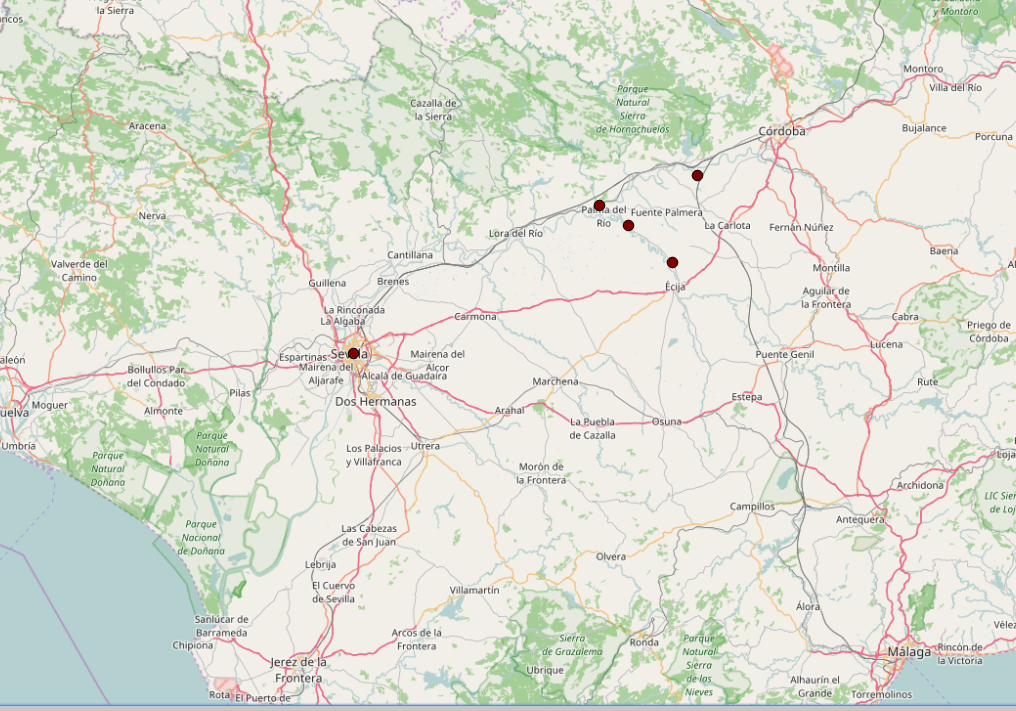
\includegraphics[scale=0.30]{romanworkshop.png}
\caption{Dressel 20 workshops were mostly distributed along the rivers Gualdalquivir and Genil. Location of the five workshops analyzed in this area.}
\label{romanworkshop}
\end{figure} 


We created a dataset where were selected 80-100 samples of each pottery workshops. The choice of these workshops corresponded to several reasons. Firstly, the workshops were selected from different spaces in order to analyse the production patterns depending on the distance of each workshop. Secondly, the extended chronology of these workshops serves as proxy to examine changes on the variation shape. In our case, the type Dressel 20 did not experimented especially visible changes on the production pattern during almost three centuries \citep{berni_dressel_2016}. Finally, the workshops selected were open excavated and provided a large number of materials.   

Eight different measurements were taken for each amphorae sample of the 5 workshops studied. The measurements were focused on the rim sherds whose fragments were the most preserved on the archaeological sample. In the case of pottery attributes, rim sherds and the curvature of handles work as an useful indicators of variability \citep{berni_millet_epigrafianforica_2008}.
The measurements were divided into exterior diameter, inside diameter, rim height, rim width, shape width, rim inside height, other rim width and protruding rim, as the Fig~\ref{mesures} indicates. The method required a large sample size and for this reason the test was focused on rim sherds. Other significant parts such as handles and bases were found in lesser quantities thus compromising the applicability of the method due to small sample size.

\begin{figure}[htp]
	\centering
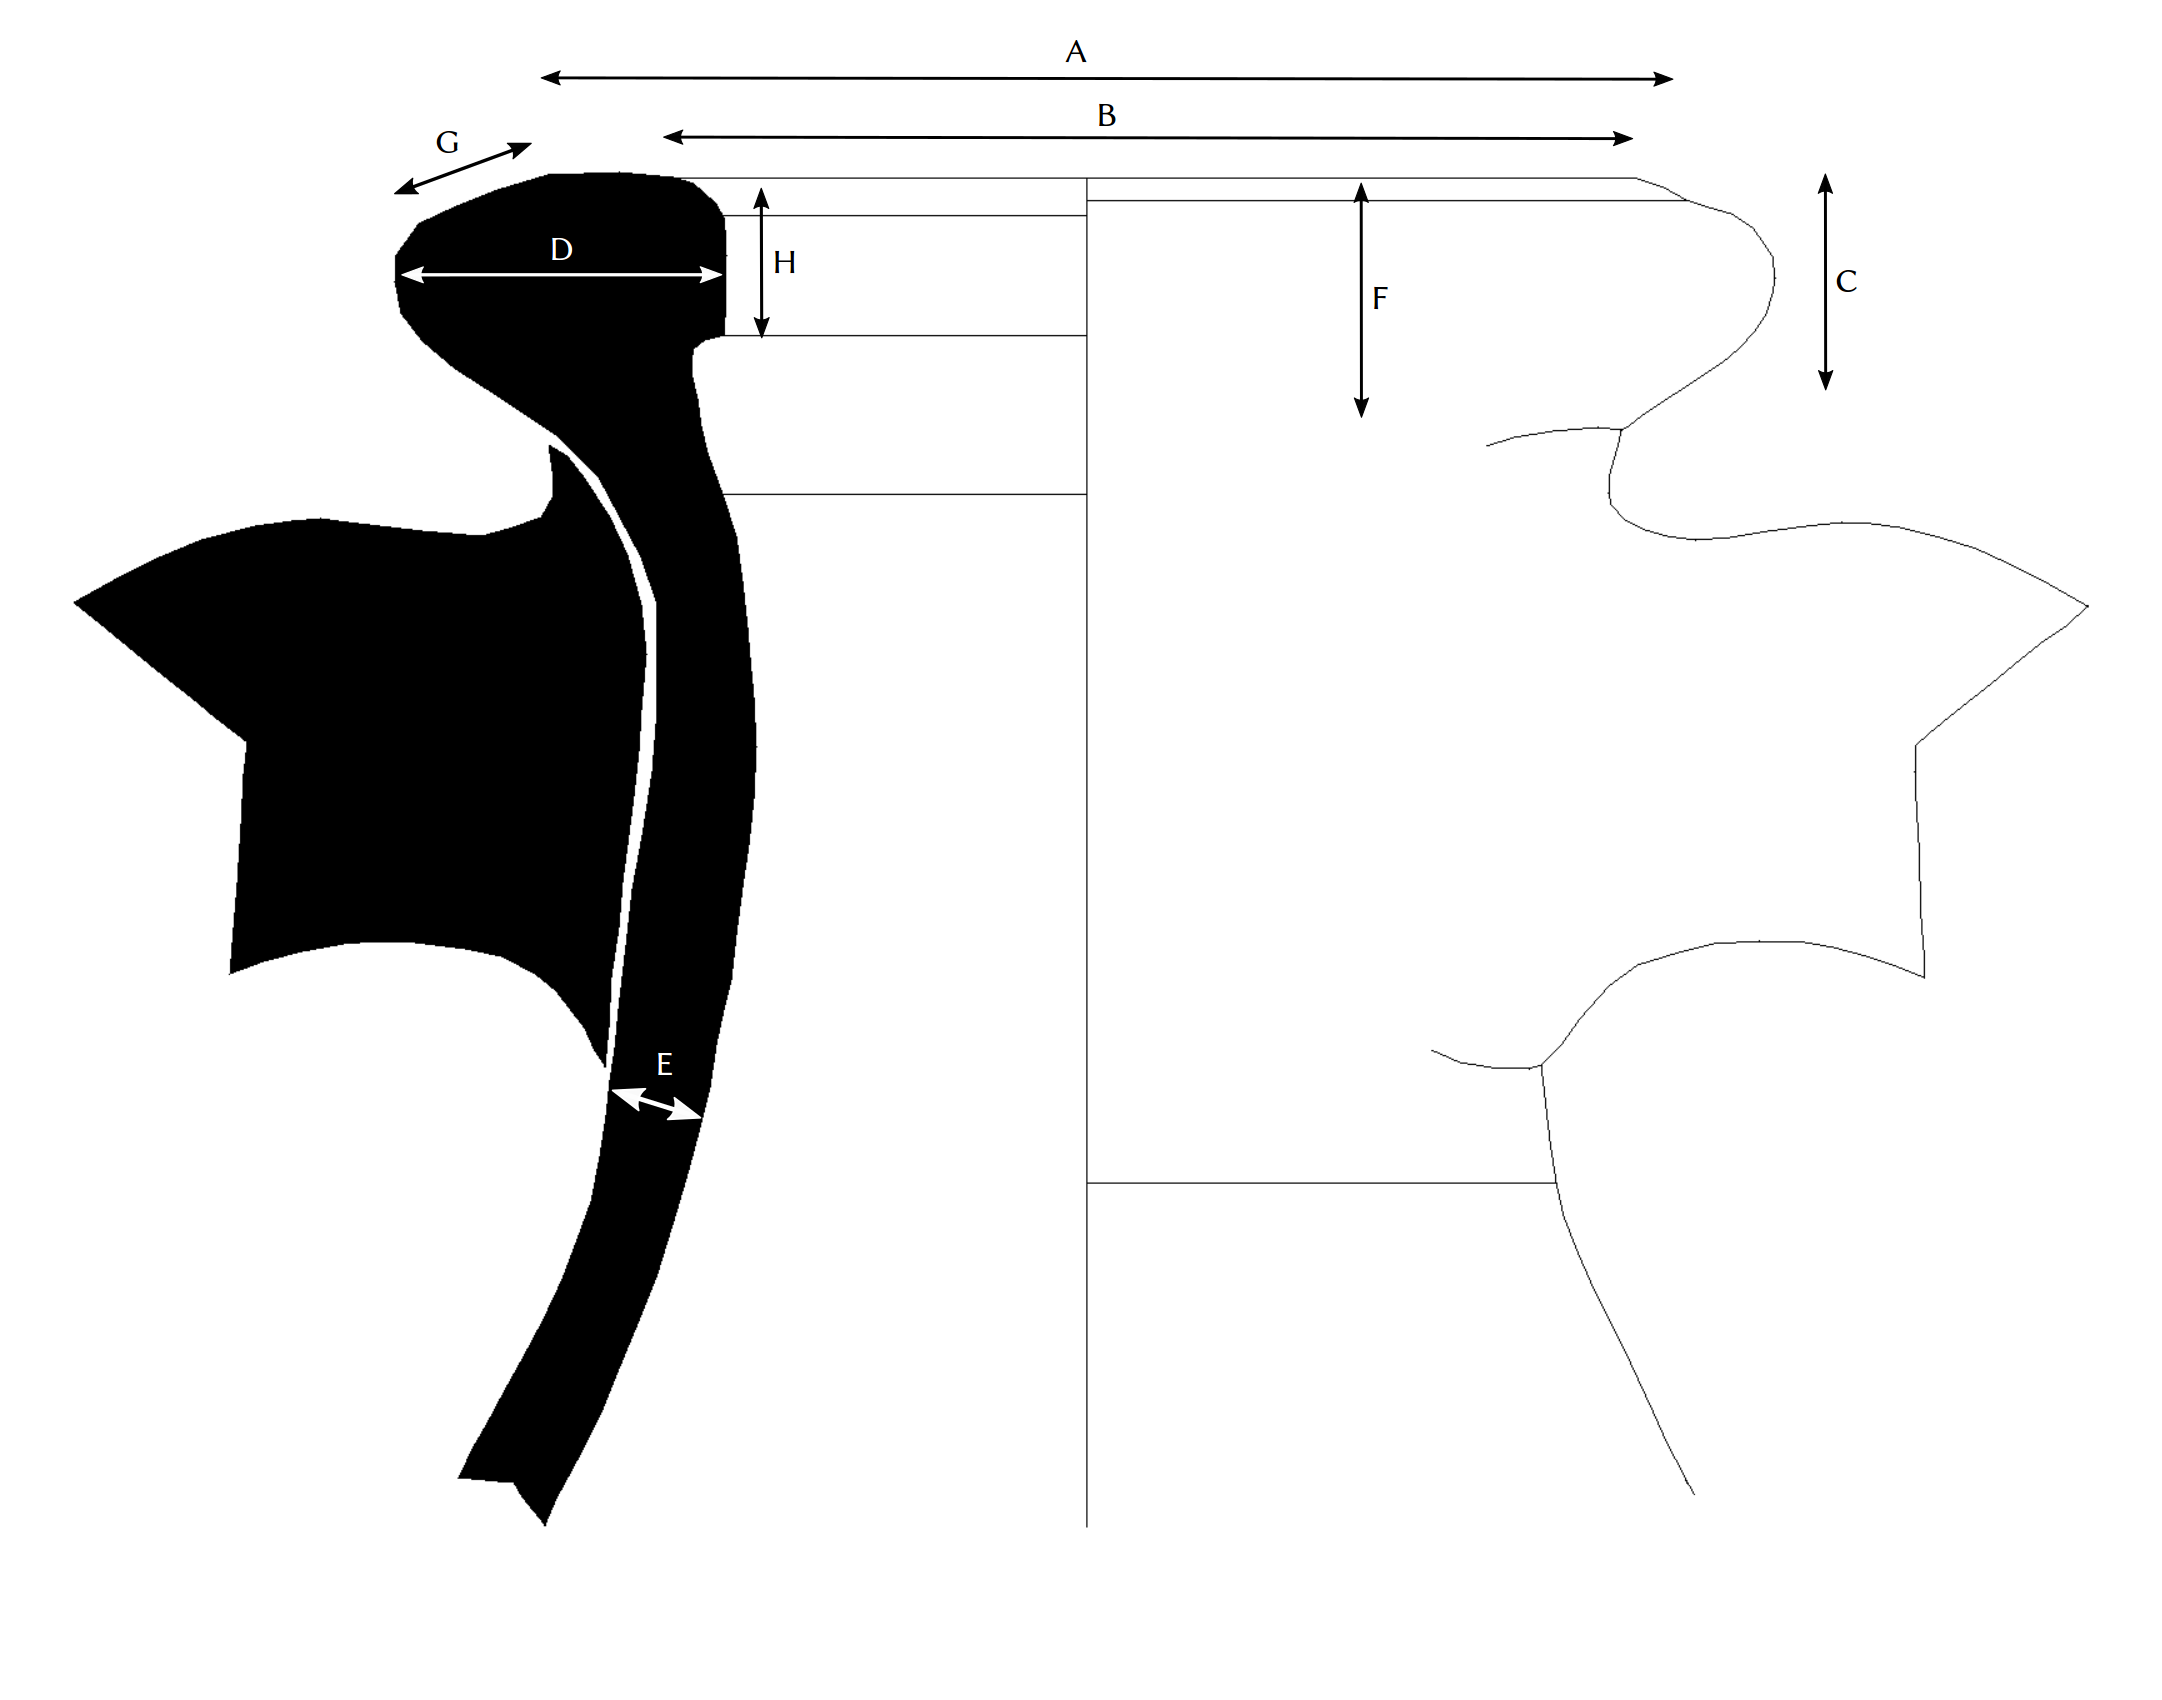
\includegraphics[scale=0.10]{mesures.png}
\caption{Example of the 8 measurements taken for the sample in order to provide morphometric data. A: external diameter. B: inside diameter. C: Rim height. D: Rim width. E: shape width. F: rim inside height. G: rim width 2. H: protruding rim}
\label{mesures}
\end{figure} 

In our study, we have selected five variants according with three centuries
(Dressel C: I-II; Dressel D: II; Dressel E: III). Without important variations in three centuries, the chronology respond to a relative dating obtained by the classification identified on shapes in different studies defined by defined by P. Berni \citep{berni_millet_epigrafianforica_2008} and Martin Kilcher \citep{martin-kilcher_romischen_1994}. All of the variants selected were found in excavations from the proper workshops studied in order to avoid some material which can contaminate the sample. For the proposal of this study, the rest of variants were not taken into account from our study by not having enough material for the analysis. 


\subsection{Principal Component Analysis}

The sample selected were analyzed using statistical method such as Principal Component Analysis and Discriminant Analysis to explore these metrical differences on the rim sherds.
We used Principal Component Analysis (PCA) to simplify the large number of variables in our dataset. This method allows to capture the most of variation from our dataset and create a reduced number of new variables without losing relevant information \citep{jolliffe_principal_2002, shennan_quantifying_1997}. Moreover the new set of variables contain all the data information expressed as the result of the most variance from the original variables. This method is commonly used in archaeology for the study of the variation of material culture \citep{li_crossbows_2014, schillinger_differences_2016}. In our study, this method allowed to capture the most variation of the measurement and retained into two firsts principal components. 

%The new set of variables contain all the relevant information of the previous variables without losing relevance. The firsts principal components are expressed as the result of the most variance of the all information from the original variables. Moreover the information is expressed as the result of most variation retained in the first principal components \citep{jolliffe_principal_2002, shennan_quantifying_1997}. of the measurements and  into PCs and take the firsts PCA with more variability in the dataset. 

\maria{Revisar}

\subsection{Discriminant Linear Analysis} 

The variability of the first 2 Principal Components was used to cluster our dataset using Linear Discriminant Analysis (LDA). LDA will be conducted to find significant differences among workshops by the combination among variables obtained for the firsts principal components. LDA identifies which variables allow to distinguish each group and how many variables are necessary to achieve the best combination as possible. Thus, LDA is used to explore a better separate training set from the results of the most relevant principal components. In our dataset, the firsts principal components produced by the amphorae measurements are grouped into each workshop groups and are separated to obtain a better discrimination among groups. 
We also generate a Confusion Matrix (CM) to able of quantifying the degree of confusion and compare the index of similarity among workshops.  CM calculated the probability of success and error of the results. It generates a matrix where higher value are the results of an incorrect classification. As example, this method has been commonly used to detect differences in artifact production \citep{charlton_investigating_2012, thorpe_distribution_1984}, and particularly for a similar study about pottery production in \emph{Tarraconense} \citep{i_martin_alisis_1998}

%The variability of the first 2 Principal Components was used to cluster our dataset using Linear Discriminant Analysis (LDA). LDA was conducted to find significant differences among workshops by the combination among variables obtained for the first principal components. LDA identifies which variables allow to distinguish or discriminate each group and how many variables are necessary to achieve the best combination as possible. In our case, this method allowed to demonstrate the correlation between spatial distance and distance among workshops. LDA was used to explore a better separate training set from the results of the most relevant principal components. LDA can classify the PCs result of the measurements into different groups.  We also generate a Confusion Matrix (CM) to able of quantifying the degree of confusion and compare the index of similarity among workshops.  CM calculated the probability of success and error of the results. It generates a matrix where higher value are the results of an incorrect classification. The distance generated with the results of DA will be compared with the spatial distance to see if it exists a correlation between morphometric distance and spatial distance. As example, this method has been commonly used to detect differences in artifact production \citep{charlton_investigating_2012, thorpe_distribution_1984}, and particularly for a similar study about the production pottery in \emph{Tarraconense} \citep{i_martin_alisis_1998}

%\xavi{El parrafo es un poco caotico. Mira otros papers para ver un poco como organizarlo mejor si puedes. Por ejemplo, no hace falta que menciones la distancia espacial hasta el final, porque en el LDA y el PCa no se usa esa distancia para nada. Quizas una subsection final sobre comparacion de distancias?}

\subsection{Distance}


\section{Results}

Several multivariate methods such as PCA and LDA were used to quantify the technical differences on the pattern production among workshops. \xavi{esta frase no anyade nada no? Hay varias mas por todo el texto...tienes que ser concisa y evitar texto que no aporte nada: }The analysis of PCA produces a set of values for each variable observed. Variables show how much variability exist in the dataset grouped by each principal components. The results, indicated in the Table~\ref{table:variable}, show the most differences were focused on the protruding rim and rim width 2. 

\begin{table}[htp]
\begin{tabular}{lcccccccc}
\hline
 Variables		&        PC1 & PC2	& PC3 & PC4 & PC5 & PC6 & PC7 & PC8     \\ \hline
 Exterior diameter	& 		 &		&	  &  	&	  &	    &     &           \\
 Inside diameter  	& 		 &		&	  &   	&	  &	    &     &           \\
 Rim height          &        &      &     &     &     &     &     &           \\
 Rim width        	&		 &		&	  &  	&	  &		&	  &          \\
 Shape width         &		 &		&	  &  	&	  &		&     &          \\
 Rim inside          &		 &	    &	  &     &	  &		&	  &          \\                                    
 Rim width 2		     & 	     &	    &	  & 		&	  &		&	  &          \\	
 Protruding rim		&        &      &      &     &     &     &     &          \\
\hline
\end{tabular}
\caption{8 principal components}
\label{table:variable}
\end{table}


The patterns observed in the first 2 Principal Components were plotted to visualize the degree of variation by isolation among workshops. The results suggested than amphorae from closer workshops tend to be more similar than amphorae made in furthest workshops. In particular, the Fig \ref{pca} illustrates how the four closest workshops show variation on PC1 (i.e. Bel\'en, Delicias, Villaseca and Malpica) while Parlamento displays a distinctive pattern than the rest of workshops on PC2 values. 

\begin{figure}[htp]
	\centering
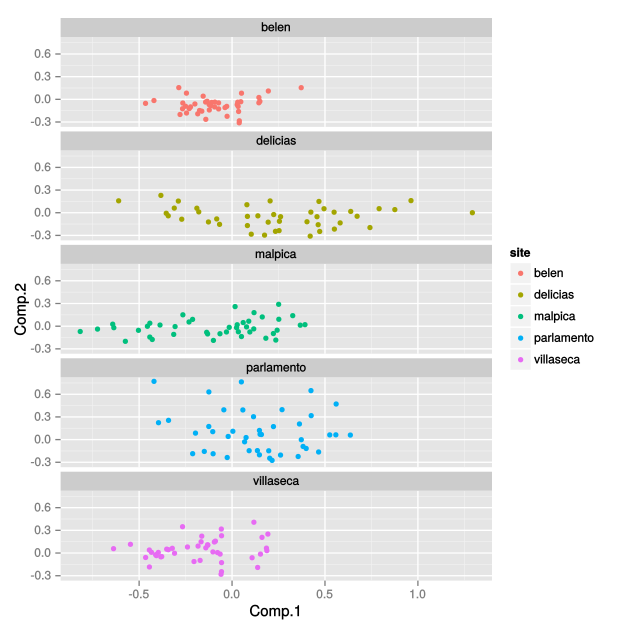
\includegraphics[scale=0.45]{pca.png}
\caption{First and Second Principal Components for the amphorae measurement dataset from the 5 workshops analyzed }
\label{pca}
\end{figure} 


\begin{table}[htp]
\begin{tabular}{lcccccccc}
\hline
      		&  PC1 & PC2	& PC3 & PC4 & PC5 & PC6 & PC7 & PC8     \\ \hline
Eigenvalue  	& 	   &		&	  &  	&	  &	    &     &           \\
Proportion  & 	   &		&	  &   	&	  &	    &     &           \\
Cumulative  &       &    &     &     &     &     &     &           \\

\end{tabular}
\caption{Result values from Principal Component Analysis}
\label{table:spatgeo}
\end{table}

Discriminant Analysis was used to analyse the results obtained from PCA. \xavi{y ya esta? Creo que haria falta ilustrar un poco mas los resultados del DA.} The results of CM proved that workshops with more troubles to be distinguished such as Malpica and Bel\'en due to the similarity on the results share a minor geographical distance than the rest (see Table~\ref{table:confusion}). Therefore, spatial distance could be inversely correlated with making techniques processes of amphorae in the case of \textit{Baetica} area. 

%\xavi{es correlacion inversa no? + distancia espacial = - similaridad de amforas}

\begin{table}[htp]
\begin{tabular}{lccccc}
\hline
 & Belen & Delicias & Malpica & Parlamento & Villaseca\\ \hline
Belen & 31 &       8 &      14 &          9 &          9 \\
Delicias       & 0 &        22 &       6&         11&         1 \\
Malpica &       5  &     2  &    11   &       2  &      10 \\
Parlamento &     4  &      5 &      6 &        15 &        5\\
Villaseca   &   3   &     6   &    6  &        6  &     18 \\
\hline

\end{tabular}
\caption{Confusion Matrix with rows pointing out the workshops analysed. The sample analyzed gave an accuracy percentage of 45.12 $\%$. Results of P.Value $<$0.01. }
\label{table:confusion}
\end{table}


We compared morphometric and spatial distance by performing peer-to-peer analysis between all the workshops. We calculated the geographical distance between each site and the distance among amphora measurements, calculated using the previous results. The workshops were chosen with different distance in order to prove the correlation between spatial distance and variability of the amphorae. Distance Matrix (see Table~\ref{table:spatialdistance}) shows the results of the analysis of morphometric distance. The workshops with morphometric distances lower tended to be more similar than the rest. The results of the analysis were compare with the real geographic distance, shown in the Table~\ref{table:spatgeo}. Here morphometric distance of the amphorae are strongly correlated with the spatial distance of workshops. When geographic distance is lower as the example of Belen and Malpica the morphometric distance is more similar whereas when distance is higher, as Parlamento, the morphometric distance display differences with the rest of workshops. Thus, the results suggest a variability on the making-techniques processes might depend on the spatial distance.  


\begin{table}[htp]
\begin{tabular}{lccccc}
\hline
 & Belen & Delicias & Malpica & Parlamento & Villaseca\\ \hline
Belen &  &        &         &           &           \\
Delicias       &   &        &       &         &          \\
Malpica &          &        &          &         &       \\
Parlamento &        &         &       &         &        \\
Villaseca   &       &        &      &          &      \\
\hline

\end{tabular}
\caption{Results of matrix distance among workshops}
\label{table:spatialdistance}
\end{table}



\begin{table}[htp]
\begin{tabular}{llcc}
\hline
 From		& To 		& Morphometric distance	& Geographic distance\\ \hline
 Parlamento	& Belen		& 						&  72.45				 \\
 Parlamento	& Delicias	& 						&  82.01				 \\
 Parlamento	& Malpica   &                       	&  74.77                      \\
 Parlamento	& Villaseca	&						&  95.33					\\
 Belen		& Parlamento &						&  72.45						\\
 Belen		& Delicias   &						&  22.82      				 \\                                    
 Belen		& Malpica	&						&  8.73							\\	
 Belen		& Villaseca  &                       &  25.23                         \\
 Delicias	& Parlamento  &                      &  82.01                            \\
 Delicias	& Belen       &						&  22.82						\\
 Delicias	& Malpica     &						&  14.19						\\
 Delicias	& Villaseca   &						&  22.45						\\
 Malpica		& Parlamento  &						&  74.77						\\
 Malpica		& Belen       &						&  8.73						\\
 Malpica		& Delicias    &						&  14.19						\\
 Malpica    & Villaseca	  &						&  20.97                     \\
 Villaseca	& Belen       &						&  25.23					     \\	             Villaseca	& Malpica     &						&  20.97								\\
 Villaseca	& Delicias	  &						&  22.45								\\
 Villaseca	& Parlamento	  &						&  95.33								\\
                                                   
\hline

\end{tabular}
\caption{Results with the comparison between morphometric distance and geographic distance (km) }
\label{table:spatgeo}
\end{table}

\xavi{Y un grafico aqui en lugar de la tabla a pelo?}

\section{Discussion and Conclusion}


Differences on the making techniques processes among workshops show a variability correlated with spatial distance. The analysed morphometric traits suggest that the similarity between amphorae decrease with the spatial distance between the workshops where they were produced. As result, amphorae made in nearby workshops with a minor spatial distance share more traits than amphorae made in pottery workshops furthest. In other words, the variability on the making techniques processes between closer workshops was difficult to differentiate. In our case, Malpica and Bel\'en workshops where the geographical proximity are the closest shared more traits in comparison with other workshops (Parlamento and Las Delicias). Thus the probability of interaction between workshops is increasing when the proximity is closest while this likelihood decreases when the possibility of interaction is low. 

We have observed than rivers courses could have affected in the transmission factors. In the case of the commerce, rivers and its tributaries played an important role for the transport of goods. The huge demand within Roman Empire and the good conditions for the loading and unloading of products \citep{bevan_mediterranean_2014} might have influenced the mode of transmission due to the continuous contact between workshops. 

The results suggest also that vertical transmission could be the main cultural mechanism to explain the variability between workshops. The different morphological traits among workshops seem proper of a low contact between potters from others workshops. The evidenced confirms therefore that these techniques traits were transmitted with high fidelity and only with few changes during three centuries. It would mean that the disciples could have remained the making techniques processes in the workshops where they were trained.  

By contrast, horizontal transmission doesn't seem to be the most probable process. The continuous contact between potters from different places had generated a more homogeneity in the technical practises. Workshops were sharing the same production techniques. As result, it would generate a social network where potters with the same social learning level worked in different workshops at the same time. Our result suggest a progressive contact with closer workshop instead. Moreover, the fact that isolation by distance is detected suggests a limited displacement between distant workshops. Thus, vertical transmission would be explained with this observed process. However, the diversity of social learning processes are clearly complex. In other words, the transmission of knowledges between master and disciple did not discard that horizontal transmission played an important role in this process as well. It can be a process where this vertical transmission dominated at first in the same workshops but consequently this transmission would be affected by workers who exchanged ideas or workers moving to other workshops.  

%podría ser conclusión
The combination of empirical analysis with the statistical methods have provided a strong baseline for a better understanding of the amphorae production in the Roman Empire. These methods offer also an strong complement to other methods as archaeometry for the characterization of production sites and places of consumption.  

We have identified measurable differences in the techniques by observing and we have tested these particularities using multivariate methods. Our analysis provides an useful baseline for the exploration of the social learning processes related with amphora production in the Roman Empire. Hence, the results have lightened to understand the link between social learning and archaeological evidence in a diversity of scenarios. 

\section{Acknowledgments}

The research was funded by European Research Council Advanced Grant EPNet (340828).
We are grateful to Enrique Garc\'ia-Vargas, ETC.  Data were collected and performed and analysed in R version 3.2.4. statistical language and implemented with the package MASS.
\maria{incluir la url con los datos y el código and citation needed}



%\section{Bibliography styles}

%There are various bibliography styles available. You can select the style of your choice in the preamble of this document. These styles are Elsevier styles based on standard styles like Harvard and Vancouver. Please use Bib\TeX\ to generate your bibliography and include DOIs whenever available.

\section*{References}

%\bibliographystyle{apalike}
\bibliography{mybibfile}

\end{document}

\cite
